\subsection{Ermittlung der Einfügedämpfung} \label{subsec:ermittlung}
In diesem Kapitel wird erläutert, wie von den Schaltungen für Gegentakt und Gleichtakt, die Einfügedämpfung(engl. Insertion Loss, IL) berechnet wird. Unteranderem wird Modular beschrieben, wie die Berechnungen im Model der Software implementiert ist. \\

Die Einfügedämpfung ist eine Grösse, die verwendet wird, um das Verhalten einer Schaltung zu beschreiben. In diesem Fall handelt es sich um ein EMI-Filter. Sie beschreibt das Verhältnis zwischen der eingehenden Leistung zur abgegebenen Leistung. Es handelt sich um eine logarithmische Grösse. Um die Einfügedämpfung in einem Bereich von bis 30MHz abzudecken wird die Formel \ref{equ:Einfügungsverluste} verwendet. In der Formel \ref{equ:Einfügungsverluste} wird die Einfügedämpfung mittels Streuparameter(S-Parameter) berechnet. Die Streuparameter werden im Anhang(Verweis) ausführlich beschrieben. Der Streuparameter $S_{21}$ beschreibt im wesentlichen den Transmissionsgrad des eingehenden Signals. Der Transmissionsgrad beschreibt, welchen Anteil des eingehenden Signals am Ausgang wieder herauskommt. \\

\begin{equation}\label{equ:Einfügungsverluste}
	IL = -20*log (\left\lvert S_{21} \right\rvert)
\end{equation}

Die Einfügedämpfung wird auf Gleichtakt und Gegentakt aufgetrennt. Dieses Prinzip ist eine gängige Methode und wird im Anhang(Verweis) ausführlich beschrieben. Für die beiden Schaltungen, welche der Aufgabenstellung(Verweis Aufgabenstellung) entnommen wurden, werden die S-Parameter berechnet. Damit dies möglich ist, wurden die Schaltungen weitgehend vereinfacht. Dies wird im Anhang(Verweis) Schritt für Schritt beschrieben. Aus den Vereinfachungen gehen folgende Schaltungen hervor(Abbildung \ref{fig:cmschaltung}, \ref{fig:dmschaltung}).

\begin{figure}[H]
		\centering
		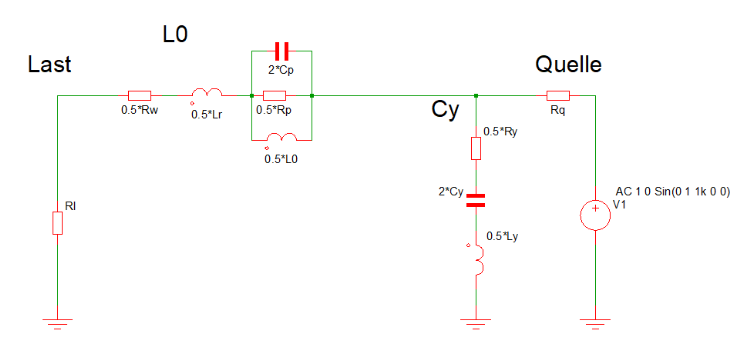
\includegraphics[width = 9cm]{EMI_CMvereinfacht.png}
		\label{fig:cmschaltung}
		\caption{reduzierte Gleichtaktschaltung}
\end{figure}

\begin{figure}[H]
		\centering
		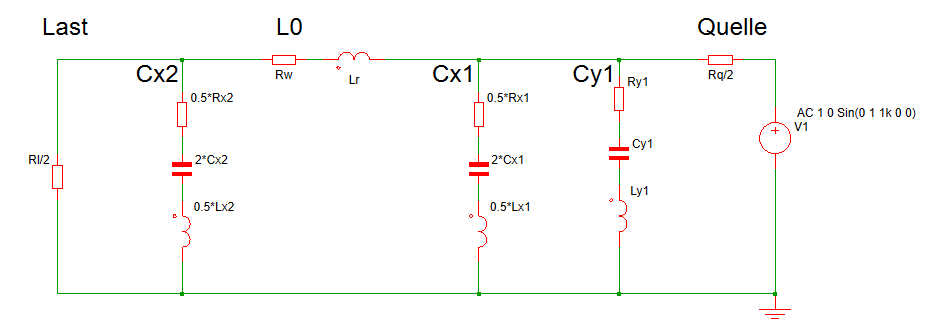
\includegraphics[width = 9cm]{EMI_DMvereinfacht.png}
		\label{fig:dmschaltung}
		\caption{reduzierte Gegentaktschaltung}
\end{figure}

Um die beiden Schaltungen anhand der Streuparameter zu beschreiben, werden die einzelnen Schaltungsteile anhand von Kettenmatrixen beschrieben(siehe Anhang Verweis Kettenmatrix). Wie im Anhang(Verweis Längs- Querimpedanz) beschrieben werden dazu die Kettenmatrixen für Längsimpedanzen und Querimpedanzen verwendet. Dies führt dazu, dass die einzelnen Schaltungsteile entweder eine Längsimpedanz oder eine Querimpedanz bilden müssen. Die Aufteilung der einzelnen Schaltungsteilen in ist in den Abbildungen (Verweis Aufteilung 1 und 2) grafisch dargestellt, wobei „LI“ eine Längsimpedanz kennzeichnet und „QI“ eine Querimpedanz. (%TODO Schaltungsteile einzeichnen)\\
\begin{figure}[H]
		\centering
		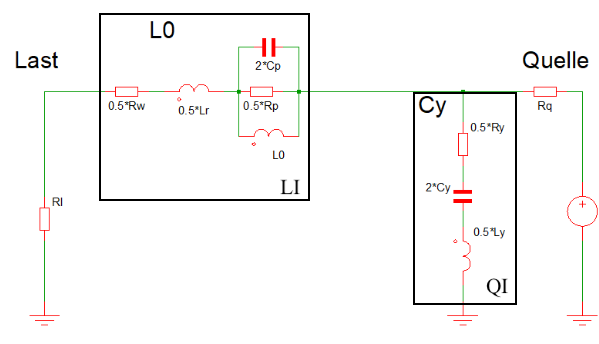
\includegraphics[width = 9cm]{EMI_CMvereinfacht_markiert.png}
		\label{fig:cmschaltung}
		\caption{Einteilung der Gleichtaktschaltungteile}
\end{figure}

\begin{figure}[H]
		\centering
		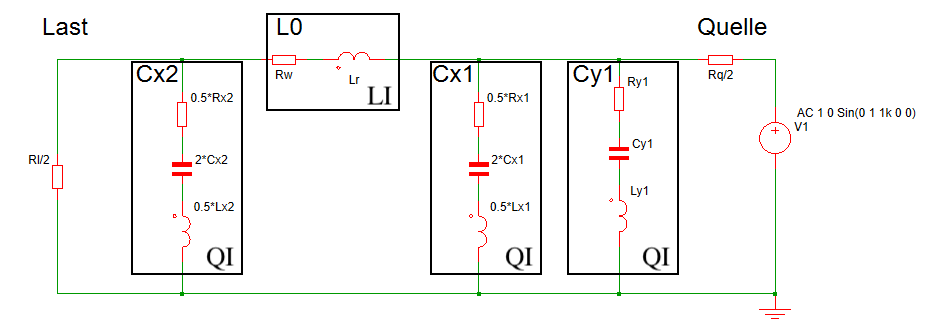
\includegraphics[width = 9cm]{EMI_DMvereinfacht_markiert.png}
		\label{fig:dmschaltung}
		\caption{Einteilung der Gegentaktschaltungsteile}
\end{figure}

Im nächsten Schritt werden die Impedanzen der einzelnen Schaltungsteile gebildet, welche in die passenden Kettenmatrixen eingesetzt werden. Um die Kettenmatrixen der Gesamtschaltungen zu bilden, werden die einzelnen Kettenmatrixen durch Kaskadieren zusammengefasst(Verweis Theoretische Grundlagen: Kettenmatrix). Die Kaskadierung entspricht im wesentlichen der Matrixmultiplikation der Kettenmatrixen. \\

\begin{equation}\label{equ:s21ausAMatrix}
s_{21} = \frac{2}{A_{11}+\frac{A{12}}{R_w}+A_{21}*R_w+A_{22}}
\end{equation}

Anhand der Kettenmatrixen der beiden Schaltungen, wird mit der Formel \ref{equ:s21ausAMatrix} der Streuparameter $S_{21}$ berechnet. A1 bis A4 entsprechen den einzelnen Einträge der Matrix. $R_w$ ist die Bezugsimpedanz. Die Bezugsimpedanz bezieht sich auf die Innenimpedanz der Quelle und die Lastimpedanz. Bezüglich der Aufgabenstellung(Verweis Aufgabenstellung) ist dieser auf 50Ohm festgelegt. Ausserdem ist es wichtig, dass die beiden Impedanzen gleich gross sind damit die Schaltung Reziprok ist(Verweis Theoretische Grundlagen: Reziproke Schaltungen). (Wieso ?) 
Bei der reduzierten Gegentaktschaltung (Abbildung \ref{fig:dmschaltung}) werden die beiden Impedanzen mit 25Ohm aufgeführt. Dies ergibt sich durch das Zusammenfassen der Gegentaktschaltung.\\

